\documentclass[xcolor={dvipsnames,svgnames,table}]{beamer}

\usepackage{../common/python}
\usepackage{amsmath}
\usepackage{centernot}
\usepackage{etoolbox}
\usepackage{mathtools}
\usepackage{slides}
\usepackage{stmaryrd}
\usepackage{tikz}

\usetikzlibrary{arrows}
\usetikzlibrary{backgrounds}
\usetikzlibrary{calc}
\usetikzlibrary{positioning}

\newcommand{\bankdistance}{4}
\tikzstyle{bank}=[
  draw,
  minimum width=1.5cm,
  minimum height=1cm,
  font=\huge
]
\tikzstyle{op}=[
  ->,
  ultra thick
]

\newcommand{\drawbanks}[6]{{
  \newcommand{\banka}{#1}
  \newcommand{\bankb}{#2}
  \newcommand{\bankaa}{#3}
  \newcommand{\bankbb}{#4}
  \newcommand{\bankaaa}{#5}
  \newcommand{\bankbbb}{#6}

  \node[bank, label=above:{Replica $A$}] (a1) at (0,              0) {\banka};
  \node[bank                           ] (a2) at (0,             -3) {\bankaa};
  \node[bank                           ] (a3) at (0,             -6) {\bankaaa};
  \node[bank, label=above:{Replica $B$}] (b1) at (\bankdistance,  0) {\bankb};
  \node[bank                           ] (b2) at (\bankdistance, -3) {\bankbb};
  \node[bank                           ] (b3) at (\bankdistance, -6) {\bankbbb};

  \draw[op] (a1) -- (a2);
  \draw[op] (a2) -- (a3);
  \draw[op] (b1) -- (b2);
  \draw[op] (b2) -- (b3);
}}

\newcommand{\zigzag}[2]{{
  \newcommand{\banka}{#1}
  \newcommand{\bankb}{#2}

  \draw[red, op] ($(\banka) + (0, -0.7)$) -- ($(\bankb) + (0, -1.0)$);
  \draw[red, op] ($(\bankb) + (0, -1.0)$) -- ($(\banka) + (0, -1.3)$);
  \draw[red, op] ($(\banka) + (0, -1.3)$) -- ($(\bankb) + (0, -1.6)$);
  \draw[red, op] ($(\bankb) + (0, -1.6)$) -- ($(\banka) + (0, -1.9)$);
}}

% Implication.
\tikzstyle{impl}=[-implies, double distance=3pt]

% Transaction.
\tikzstyle{txn}=[ultra thick, ->]

% Derived transaction.
\tikzstyle{dtxn}=[ultra thick, ->, dashed]

% Invariant node.
\newcommand{\inode}[3][]{
  \node[draw, shape=circle, minimum width=0.5cm, #1] (#2) at (#3) {};
  \node[fill, shape=circle, #1] () at (#3) {};
}

% Normal node.
\newcommand{\nnode}[3][]{
  \node[fill, shape=circle, #1] (#2) at (#3) {};
}


\newcommand{\dbs}{\mathcal{D}}
\newcommand{\var}{\textsf{Var}}
\newcommand{\ints}{\mathbb{Z}}

\newcommand{\wimp}{W$\iinvariant$MP}
\newcommand{\imp}{$\iinvariant$MP}
\newcommand{\impaexp}{\textsf{Aexp}}
\newcommand{\impbexp}{\textsf{Bexp}}
\newcommand{\impcom}{\textsf{Com}}
\newcommand{\impskip}{\textsf{skip}}
\newcommand{\impif}[3]{\textsf{if}(#1)\set{#2}\textsf{else}\set{#3}}

\newcommand{\iinvariant}{\mathcal{I}}
\newcommand{\iconfluent}{$\iinvariant$-confluent}
\newcommand{\iconfluence}{$\iinvariant$-confluence}
\newcommand{\ipreservation}{$\iinvariant$-preservation}
\newcommand{\ipreserving}{$\iinvariant$-preserving}
\newcommand{\isafety}{$\iinvariant$-safety}
\newcommand{\isafe}{$\iinvariant$-safe}
\newcommand{\istrength}{$\iinvariant$-strength}
\newcommand{\istrong}{$\iinvariant$-strong}
\newcommand{\istrengthstar}{\istrength$^\ast$}
\newcommand{\istrongstar}{\istrong$^\ast$}
\newcommand{\iconvergence}{$\iinvariant$-convergence}
\newcommand{\iconvergent}{$\iinvariant$-convergent}


\newcommand{\defeq}{\stackrel{\mathclap{\normalfont\mbox{\scriptsize def}}}{=}}
\newcommand{\denote}[1]{\left\llbracket#1\right\rrbracket}
\newcommand{\set}[1]{\left\{#1\right\}}

\title{Enforced \iconfluence{}}
\author{Michael Whittaker}
\date{September 29, 2017}

\begin{document}
\begin{frame}
  \maketitle
\end{frame}

\begin{frame}{Coordinating}
  \begin{center}
    \begin{tikzpicture}
      \drawbanks{\$50}{\$50}
                {\$60}{\$60}
                {\$80}{\$80}

      \draw[op] ($(a1) + (-2, 0)$) -- (a1) node[midway, above] {$+\$10$};
      \draw[op] ($(b1) + (+2, 0)$) -- (b1) node[midway, above] {$+\$20$};
      \draw[op] (a2) -- ($(a2) + (-2, 0)$) node[midway, above] {OK};
      \draw[op] (b3) -- ($(b3) + (+2, 0)$) node[midway, above] {OK};

      \zigzag{a1}{b1}
      \zigzag{a2}{b2}
    \end{tikzpicture}
  \end{center}
\end{frame}

\begin{frame}{Coordinating}
  \begin{center}
    \begin{tikzpicture}
      \drawbanks{\$50}{\$50}
                {\$20}{\$20}
                {\$20}{\$20}

      \draw[op] ($(a1) + (-2, 0)$) -- (a1) node[midway, above] {$-\$30$};
      \draw[op] ($(b1) + (+2, 0)$) -- (b1) node[midway, above] {$-\$40$};
      \draw[op] (a2) -- ($(a2) + (-2, 0)$) node[midway, above] {OK};
      \draw[op] (b3) -- ($(b3) + (+2, 0)$) node[midway, above] {NO};

      \zigzag{a1}{b1}
      \zigzag{a2}{b2}
    \end{tikzpicture}
  \end{center}
\end{frame}

\begin{frame}{Avoiding Coordination}
  \begin{center}
    \begin{tikzpicture}
      \drawbanks{\$50}{\$50}
                {\$60}{\$70}
                {\$80}{\$80}

      \draw[op] ($(a1) + (-2, 0)$) -- (a1) node[midway, above] {$+\$10$};
      \draw[op] ($(b1) + (+2, 0)$) -- (b1) node[midway, above] {$+\$20$};
      \draw[op] (a2) -- ($(a2) + (-2, 0)$) node[midway, above] {OK};
      \draw[op] (b2) -- ($(b2) + (+2, 0)$) node[midway, above] {OK};

      \draw[dashed, op] (a2) -- (b3) node[near start, sloped, above] {$+\$10$};
      \draw[dashed, op] (b2) -- (a3) node[near start, sloped, above] {$+\$20$};
    \end{tikzpicture}
  \end{center}
\end{frame}

\begin{frame}{Avoiding Coordination}
  \begin{center}
    \begin{tikzpicture}
      \drawbanks{\$50}{\$50}
                {\$20}{\$10}
                {-\$20}{-\$20}

      \draw[op] ($(a1) + (-2, 0)$) -- (a1) node[midway, above] {$-\$30$};
      \draw[op] ($(b1) + (+2, 0)$) -- (b1) node[midway, above] {$-\$40$};
      \draw[op] (a2) -- ($(a2) + (-2, 0)$) node[midway, above] {OK};
      \draw[op] (b2) -- ($(b2) + (+2, 0)$) node[midway, above] {OK};

      \draw[dashed, op] (a2) -- (b3) node[near start, sloped, above] {$-\$30$};
      \draw[dashed, op] (b2) -- (a3) node[near start, sloped, above] {$-\$40$};
    \end{tikzpicture}
  \end{center}
\end{frame}

\begin{frame}{\iconfluence{}}
  \begin{columns}
    \begin{column}{0.5\textwidth}
      \frame{
        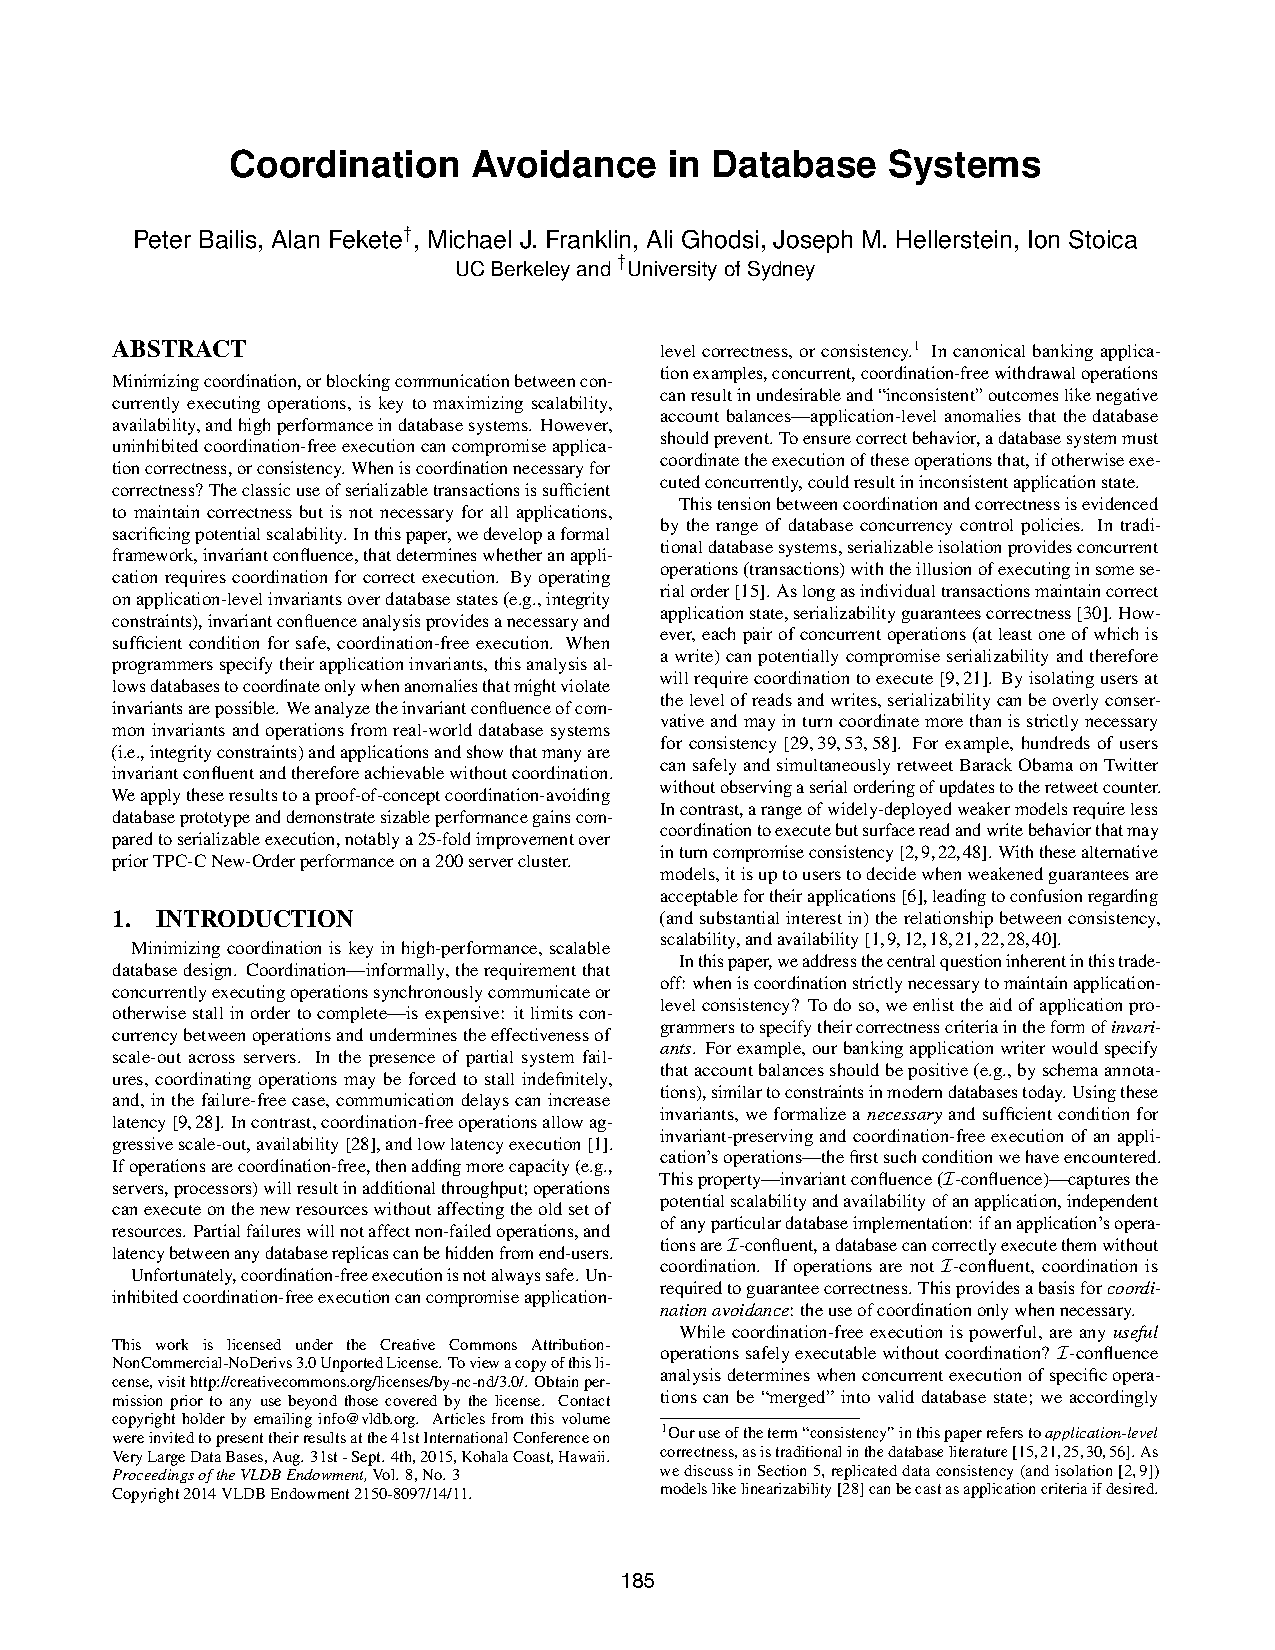
\includegraphics[width=\textwidth]{figs/bailis-iconfluence-page1.pdf}
      }
    \end{column}
    \begin{column}{0.5\textwidth}  %%<--- here
      \begin{center}
        A set of of transactions $T$ is \emph{invariant-confluent}
        (\iconfluent) with respect to $I$ if and only if $T$ can execute
        without coordination while preserving $I$.
      \end{center}
    \end{column}
  \end{columns}
\end{frame}

\begin{frame}{\iconfluence{}}
  \begin{center}
    \begin{tikzpicture}
      \newcommand{\proofa}{proof17}
      \newcommand{\proofb}{proof12}
      \newcommand{\proofc}{proof16}
      \newcommand{\proofwidth}{5cm}

      \node[draw, fill=white] (\proofa) at (0, 0) {
        \includegraphics[width=\proofwidth]{figs/\proofa.pdf}
      };
      \node[draw, fill=white] (\proofb) at (\proofa.south east) {
        \includegraphics[width=\proofwidth]{figs/\proofb.pdf}
      };
      \node[draw, fill=white] (\proofc) at (\proofb.south east) {
        \includegraphics[width=\proofwidth]{figs/\proofc.pdf}
      };
    \end{tikzpicture}
  \end{center}
\end{frame}

\begin{frame}[fragile]{Vision}
  \begin{center}
    \begin{Python}[gobble=6]
      x = PNCounter(0)

      set_invariant(x >= 0)

      # Good!
      @transaction
      def foo():
        x.increment(42)

      # Bad!
      @transaction
      def bar():
        x.decrement(1)
    \end{Python}
  \end{center}
\end{frame}

\begin{frame}[fragile]{Vision}
  \begin{center}
    \begin{Python}[gobble=6]
      employees = Map[Int, String]()
      teams = Set[Set[Int]]

      # All ids in teams must appear in employees.
      set_invariant(forall team in teams.
        team subset employees.keys())
      # All teams must be disjoint.
      set_invariant(forall a, b in teams.
        a != b => a intersect b = {})
      # Every employee must be on a team
      set_invariant(union(teams) = employees.keys())

      @transaction
      def add_employee(name):
        id = employees.unique_id()
        employees.put(name, id)
        teams[0].add(id)
    \end{Python}
  \end{center}
\end{frame}

\newcommand{\iconfluenceintuitively}{
  \begin{frame}{\iconfluence{}, Intuitively}
    \begin{center}
      \begin{tikzpicture}[scale=1.5]
        \inode[label=above:$D$]{a}{0, 0}
        \inode[]{l1}{$(a) + (225:1)$}
        \inode[]{l2}{$(l1) + (225:1)$}
        \inode[]{l3}{$(l2) + (225:1)$}

        \inode[]{r1}{$(a) + (315:1)$}
        \inode[]{r2}{$(r1) + (315:1)$}
        \inode[]{r3}{$(r2) + (315:1)$}

        \dnode{b}{$(l3) + (315:3)$}

        \draw[txn] (a)  -- (l1) node[pos=0.3, left]  {$t_1$};
        \draw[txn] (l1) -- (l2) node[pos=0.3, left]  {$t_2$};
        \draw[txn] (l2) -- (l3) node[pos=0.3, left]  {$t_3$};
        \draw[txn] (a)  -- (r1) node[pos=0.3, right] {$u_1$};
        \draw[txn] (r1) -- (r2) node[pos=0.3, right] {$u_2$};
        \draw[txn] (r2) -- (r3) node[pos=0.3, right] {$u_3$};
        \draw[txn] (l3) -- (b)  node[midway, left]  {$t_1, t_2, t_3$};
        \draw[txn] (r3) -- (b)  node[midway, right] {$u_1, u_2, u_3$};
      \end{tikzpicture}
    \end{center}
  \end{frame}
}

\iconfluenceintuitively{}

\begin{frame}{\iconfluence{}, Formally}
  \begin{center}
    \huge
    A \emph{database state} $D: \var \to \ints$ is a total function mapping
    variables to integers.
  \end{center}
  \begin{itemize}
    \item e.g. $\var = \set{x}, D = \set{(x, 1)}$
    \item e.g. $\var = \set{x, y}, D = \set{(x, 42), (y, 100)}$
    \item e.g. $\var = \set{x, y, z}, D = \set{(x, 42), (y, 0), (z, 0)}$
  \end{itemize}
\end{frame}

\begin{frame}{\iconfluence{}, Formally}
  \begin{center}
    \huge
    An \emph{invariant} $I$ is a linear constraint over $\var$.
  \end{center}
  \begin{itemize}
    \item e.g. $\var = \set{x}, x \geq 0$
    \item e.g. $\var = \set{x}, x < 0 \lor x = 42$
    \item e.g. $\var = \set{x, y, z},
                \lnot(3x - 4y < z \lor (z = 42 \land y > z))$
    \item We denote that $D$ satisfies $I$ with $I(D)$.
  \end{itemize}
\end{frame}

\begin{frame}{\iconfluence{}, Formally}
  \begin{center}
    \huge
    A \emph{transaction} $t: \var \rightharpoonup \ints$ is a partial function
    mapping variables to integers.
  \end{center}
  We denote the application of transaction $t$ to database $D$ as $D \circ t$
  where
  \[
    (D \circ t)(x) \defeq \begin{cases*}
      D(x) + t(x) & $x \in dom(t)$ \\
      D(x)        & otherwise
    \end{cases*}
  \]
  \begin{itemize}
    \item $D \defeq \set{(x, 11), (y, 100)}$,
    \item $t \defeq \set{(x, 31), (y, -200)}$,
    \item $D \circ t = \set{(x, 42), (y, -100)}$.
  \end{itemize}
\end{frame}

\begin{frame}{\iconfluence{}, Formally}
  \begin{center}
    \huge
    A \emph{transaction chain} $C$ over transactions $T$ is a sequence of
    transactions $t_1, \ldots, t_n$.
  \end{center}
  \begin{itemize}
    \item Let $D \circ C \defeq D \circ t_1 \circ \cdots \circ t_n$.
    \item
      $C$ satisfies $I$ starting at $D$, denoted $I(C @ D)$, if for every
      prefix $C'$ of $C$, $I(D \circ C')$.
    \item
      Note $I(C@D) \implies I(D)$.
    \item
      Note $I(C@D) \implies I(D \circ C)$.
  \end{itemize}
\end{frame}

\begin{frame}{\iconfluence{}, Formally}
  \begin{center}
    \huge
    A set of transactions $T$ is \emph{\iconfluent{}} with respect to $I$ if
    for every database state $D$ and chains $C$, $C'$, if $I(D)$, $I(C@D)$, and
    $I(C'@D)$, then $I(D \circ C \circ C')$.
  \end{center}
\end{frame}

\iconfluenceintuitively{}

\newcommand{\inva}{x + y \geq 0}
\newcommand{\invb}{x - y \leq 0}
\newcommand{\invc}{y \geq 1}
\newcommand{\invd}{y \geq 3}
\newcommand{\inv}{(\inva \land \invb \land \invc) \lor (\invd)}

\begin{frame}{\iconfluence{}, Socratically}
  \begin{center}
    \begin{tabular}{c|c|c}
      $I$                 & $T$                    & \iconfluent{}? \\\hline\hline
      $x \geq 0$          & $add(x, 1)$            & \pause yes \pause \\\hline
      $x \geq 0$          & $add(x, -1)$           & \pause no  \pause \\\hline
      $x = 0$             & $add(x, 1)$            & \pause yes \pause \\\hline
      $-x + y \geq 0$     & $add(x, 1)$            & \pause no  \pause \\\hline
      $-x + y \geq 0$     & $add(x, -1)$           & \pause yes \pause \\\hline
      $-x + y \geq 0$     & $add(y, 1)$            & \pause yes \pause \\\hline
      $-x + y \geq 0$     & $add(y, -1)$           & \pause no  \pause \\\hline
      $-x + y \geq 0$     & $add(x, 1); add(y, 1)$ & \pause yes \pause \\\hline
      $x = 0 \lor y = 0$  & $add(x, 1)$            & \pause yes \pause \\\hline
      $x = 0 \lor y = 0$  & $add(y, 1)$            & \pause yes \pause \\\hline
      $x = 0 \lor y = 0$  & $add(x, 1), add(y, 1)$ & \pause no  \pause \\\hline
      $x = 0 \land y = 0$ & $add(x, 1), add(y, 1)$ & \pause yes \pause \\\hline
      %
      $\begin{pmatrix}
        \inva \land {} \\
        \invb \land {} \\
        \invc
       \end{pmatrix} \lor \invd$ & ???  & ??? \\
    \end{tabular}
  \end{center}
\end{frame}

\begin{frame}{\iconfluence{}, Goemetrically}
  \begin{itemize}
    \item
      If $|\var| = n$, we can imagine databases as points in $\ints^n$.
    \item
      We can imagine invariants as a subset of $\ints^n$.
    \item
      We can imagine transactions as $n$-vectors over $\ints$.
  \end{itemize}
\end{frame}

\newcommand{\ymin}{-1}
\newcommand{\ymax}{4}
\newcommand{\xmin}{-4}
\newcommand{\xmax}{4}
\newcommand{\drawgrid}{
  \draw[opacity=0.5] (\xmin, \ymin) grid (\xmax, \ymax);
  \draw[ultra thick] (\xmin, 0) -- (\xmax, 0);
  \draw[ultra thick] (0, \ymin) -- (0, \ymax);
}
\newcommand{\drawpoints}[1]{
  \foreach \x in {\xmin, ..., \xmax} {
    \foreach \y in {\ymin, ..., \ymax} {
      \ifboolexpr{#1}{
        \node[shape=circle, fill, opacity=0.75, inner sep=3pt] (\x-\y) at (\x, \y) {};
      }{}
    }
  }
}

\begin{frame}{\iconfluence{}, Goemetrically}
  \begin{center}
    \begin{tikzpicture}
      \drawgrid{}
      \drawpoints{bool{true}}
    \end{tikzpicture}
  \end{center}
\end{frame}

\begin{frame}{\iconfluence{}, Goemetrically}
  \begin{center}
    $y \geq 1$

    \begin{tikzpicture}
      \drawgrid{}
      \drawpoints{test{\ifnumcomp{\y}{>}{1}} or
                  test{\ifnumcomp{\y}{=}{1}}}
    \end{tikzpicture}
  \end{center}
\end{frame}

\begin{frame}{\iconfluence{}, Goemetrically}
  \begin{center}
    $y \geq 3$

    \begin{tikzpicture}
      \drawgrid{}
      \drawpoints{test{\ifnumcomp{\y}{>}{3}} or test{\ifnumcomp{\y}{=}{3}}}
    \end{tikzpicture}
  \end{center}
\end{frame}

\begin{frame}{\iconfluence{}, Goemetrically}
  \begin{center}
    $x + y \geq 0$

    \begin{tikzpicture}
      \drawgrid{}
      \drawpoints{test{\ifnumcomp{\x+\y}{>}{0}} or test{\ifnumcomp{\x+\y}{=}{0}}}
    \end{tikzpicture}
  \end{center}
\end{frame}

\begin{frame}{\iconfluence{}, Goemetrically}
  \begin{center}
    $x - y \leq 0$

    \begin{tikzpicture}
      \drawgrid{}
      \drawpoints{test{\ifnumcomp{\x-\y}{<}{0}} or test{\ifnumcomp{\x-\y}{=}{0}}}
    \end{tikzpicture}
  \end{center}
\end{frame}

\begin{frame}{\iconfluence{}, Goemetrically}
  \begin{center}
    $t_a \defeq add(x, 1); add(y, 1)$ \quad
    $t_b \defeq add(x, -1); add(y, 1)$ \quad

    \begin{tikzpicture}
      \drawgrid{}
      \drawpoints{test{\ifnumcomp{\y}{>}{1}} or test{\ifnumcomp{\y}{=}{1}}}
      \draw[txn, red]   (0-1) -- (1-2)  node[black, midway, below] {\large $t_a$};
      \draw[txn, green] (0-1) -- (-1-2) node[black, midway, left]  {\large $t_b$};
    \end{tikzpicture}
  \end{center}
\end{frame}

\begin{frame}{\iconfluence{}, Goemetrically}
  \begin{center}
    $t_a \defeq add(x, 1); add(y, 1)$ \quad
    $t_b \defeq add(x, -1); add(y, 1)$ \quad

    \begin{tikzpicture}
      \drawgrid{}
      \drawpoints{test{\ifnumcomp{\y}{>}{1}} or test{\ifnumcomp{\y}{=}{1}}}
      \draw[txn, red]   (0-1)  -- (1-2)  node[black, midway, below] {\large $t_1$};
      \draw[txn, red]   (1-2)  -- (2-3)  node[black, midway, below] {\large $t_2$};
      \draw[txn, green] (0-1)  -- (-1-2) node[black, midway, left]  {\large $u_1$};

      \pause

      \draw[txn, dashed, green]
        (2-3) -- (1-4)  node[black, midway, below] {\large $u_1$};
      \draw[txn, dashed, red]
        (-1-2) -- (0-3)  node[black, midway, left] {\large $t_1$};
      \draw[txn, dashed, red]
        (0-3) -- (1-4) node[black, midway, left]  {\large $t_2$};
    \end{tikzpicture}
  \end{center}
\end{frame}

\begin{frame}{\iconfluence{}, Goemetrically}
  \begin{center}
    $I \defeq x = y$

    \begin{tikzpicture}
      \drawgrid{}
      \drawpoints{test{\ifnumcomp{\x}{=}{\y}}}
    \end{tikzpicture}
  \end{center}
\end{frame}

\begin{frame}{\iconfluence{}, Goemetrically}
  \begin{center}
    $I \defeq x = 0 \lor y = 0$

    \begin{tikzpicture}
      \drawgrid{}
      \drawpoints{test{\ifnumcomp{\x}{=}{0}} or test{\ifnumcomp{\y}{=}{0}}}
    \end{tikzpicture}
  \end{center}
\end{frame}

\begin{frame}{\iconfluence{}, Goemetrically}
  \begin{center}
    $I \defeq x = 0 \land y = 0$

    \begin{tikzpicture}
      \drawgrid{}
      \drawpoints{test{\ifnumcomp{\x}{=}{0}} and test{\ifnumcomp{\y}{=}{0}}}
    \end{tikzpicture}
  \end{center}
\end{frame}

\begin{frame}{\iconfluence{}, Goemetrically}
  \begin{center}
    $\begin{pmatrix}
      \inva \land {} \\
      \invb \land {} \\
      \invc
     \end{pmatrix} \lor \invd$

    \begin{tikzpicture}
      \drawgrid{}
      \drawpoints{
        ((test{\ifnumcomp{\x+\y}{>}{0}} or test{\ifnumcomp{\x+\y}{=}{0}}) and
         (test{\ifnumcomp{\x-\y}{<}{0}} or test{\ifnumcomp{\x-\y}{=}{0}}) and
         (test{\ifnumcomp{\y}{>}{1}} or test{\ifnumcomp{\y}{=}{1}})) or
        (test{\ifnumcomp{\y}{>}{3}} or test{\ifnumcomp{\y}{=}{3}})
      }
    \end{tikzpicture}
  \end{center}
\end{frame}

\begin{frame}{$k$-\iconfluence{}}
  \begin{center}
    \Large
    A set of transactions $T$ is \emph{\iconfluent{}} with respect to $I$ if
    for every database state $D$ and chains $C$, $C'$, if $I(D)$, $I(C@D)$, and
    $I(C'@D)$, then $I(D \circ C \circ C')$.

    \pause
    \vspace{1cm}

    A set of transactions $T$ is \emph{$k$-\iconfluent{}} with respect to $I$
    if for every database state $D$ and chains $C$, $C'$, if $I(D)$, $I(C@D)$,
    $I(C'@D)$, $|C| \leq k$, and $|C'| \leq k$, then $I(D \circ C \circ C')$.
  \end{center}
\end{frame}

\begin{frame}{3-\iconfluence{}}
  \begin{center}
    \begin{tikzpicture}[scale=1.5]
      \inode[label=above:$D$]{a}{0, 0}
      \inode[]{l1}{$(a) + (225:1)$}
      \inode[]{l2}{$(l1) + (225:1)$}
      \inode[]{l3}{$(l2) + (225:1)$}

      \inode[]{r1}{$(a) + (315:1)$}
      \inode[]{r2}{$(r1) + (315:1)$}
      \inode[]{r3}{$(r2) + (315:1)$}

      \dnode{b}{$(l3) + (315:3)$}

      \draw[txn] (a)  -- (l1) node[pos=0.3, left]  {$t_1$};
      \draw[txn] (l1) -- (l2) node[pos=0.3, left]  {$t_2$};
      \draw[txn] (l2) -- (l3) node[pos=0.3, left]  {$t_3$};
      \draw[txn] (a)  -- (r1) node[pos=0.3, right] {$u_1$};
      \draw[txn] (r1) -- (r2) node[pos=0.3, right] {$u_2$};
      \draw[txn] (r2) -- (r3) node[pos=0.3, right] {$u_3$};
      \draw[txn] (l3) -- (b)  node[midway, left]  {$t_1, t_2, t_3$};
      \draw[txn] (r3) -- (b)  node[midway, right] {$u_1, u_2, u_3$};
    \end{tikzpicture}
  \end{center}
\end{frame}

\begin{frame}{1-\iconfluence{}}
  \begin{center}
    \begin{tikzpicture}[scale=2]
      \inode[label=above:$D$]{a}{0, 0}
      \inode[]{l1}{$(a) + (225:1)$}
      \inode[]{r1}{$(a) + (315:1)$}
      \dnode{b}{$(l1) + (315:1)$}
      \draw[txn] (a) -- (l1) node[midway, left] {$t$};
      \draw[txn] (a) -- (r1) node[midway, right] {$u$};
      \draw[txn] (l1) -- (b) node[midway, left] {$u$};
      \draw[txn] (r1) -- (b) node[midway, right] {$t$};
    \end{tikzpicture}
  \end{center}
\end{frame}


\begin{frame}
  \begin{center}
    \huge
    $1$-\iconfluence{} $\iff$ \iconfluence{}
  \end{center}
\end{frame}

\newcommand{\onescale}{1.1}
\newcommand{\baseedges}{
  \begin{scope}[on background layer]
    \draw[txn] (03) -- (13) node[midway, above]{$u_1$};
    \draw[txn] (13) -- (23) node[midway, above]{$u_2$};
    \draw[txn] (23) -- (33) node[midway, above]{$u_3$};
    \draw[txn] (03) -- (02) node[midway, left]{$t_1$};
    \draw[txn] (02) -- (01) node[midway, left]{$t_2$};
    \draw[txn] (01) -- (00) node[midway, left]{$t_3$};
    \draw[dtxn] (00) -- (30);
    \draw[dtxn] (33) -- (30);
  \end{scope}
}

\begin{frame}{1-\iconfluence{} $\implies$ \iconfluence{}}
  \begin{center}
    \begin{tikzpicture}[scale=\onescale]
      \foreach \x/\y in {
             1/3, 2/3, 3/3,
        0/2,
        0/1,
        0/0%
      } {
        \inode{\x\y}{\x, \y}
      }
      \foreach \x/\y in {0/3} {
        \inode[red]{\x\y}{\x, \y}
      }
      \nnode{30}{3, 0}
      \baseedges{}
    \end{tikzpicture}
  \end{center}
\end{frame}

\begin{frame}{1-\iconfluence{} $\implies$ \iconfluence{}}
  \begin{center}
    \begin{tikzpicture}[scale=\onescale]
      \foreach \x/\y in {
        0/3,      2/3, 3/3,
        %
        0/1,
        0/0%
      } {
        \inode{\x\y}{\x, \y}
      }
      \foreach \x/\y in {0/2, 1/3} {
        \inode[red]{\x\y}{\x, \y}
      }
      \nnode{30}{3, 0}
      \baseedges{}
    \end{tikzpicture}
  \end{center}
\end{frame}

\begin{frame}{1-\iconfluence{} $\implies$ \iconfluence{}}
  \begin{center}
    \begin{tikzpicture}[scale=\onescale]
      \foreach \x/\y in {
        0/3, 1/3,      3/3,
        0/2,
        %
        0/0%
      } {
        \inode{\x\y}{\x, \y}
      }
      \foreach \x/\y in {0/1, 1/2, 2/3} {
        \inode[red]{\x\y}{\x, \y}
      }
      \nnode{30}{3, 0}
      \baseedges{}
      \draw[txn] (02) -- (12) node[midway, above] {$u_1$};
      \draw[txn] (13) -- (12) node[midway, left]  {$t_1$};
    \end{tikzpicture}
  \end{center}
\end{frame}

\begin{frame}{1-\iconfluence{} $\implies$ \iconfluence{}}
  \begin{center}
    \begin{tikzpicture}[scale=\onescale]
      \foreach \x/\y in {
        0/3, 1/3, 2/3,
        0/2, 1/2,
        0/1%
        %
      } {
        \inode{\x\y}{\x, \y}
      }
      \foreach \x/\y in {0/0, 1/1, 2/2, 3/3} {
        \inode[red]{\x\y}{\x, \y}
      }
      \nnode{30}{3, 0}
      \baseedges{}
      \draw[txn] (02) -- (12) node[midway, above] {$u_1$};
      \draw[txn] (13) -- (12) node[midway, left]  {$t_1$};
      \draw[txn] (01) -- (11) node[midway, above] {$u_1$};
      \draw[txn] (12) -- (11) node[midway, left]  {$t_2$};
      \draw[txn] (12) -- (22) node[midway, above] {$u_2$};
      \draw[txn] (23) -- (22) node[midway, left]  {$t_1$};
    \end{tikzpicture}
  \end{center}
\end{frame}

\begin{frame}{1-\iconfluence{} $\implies$ \iconfluence{}}
  \begin{center}
    \begin{tikzpicture}[scale=\onescale]
      \foreach \x/\y in {
        0/3, 1/3, 2/3, 3/3,
        0/2, 1/2, 2/2,
        0/1, 1/1,
        0/0%
      } {
        \inode{\x\y}{\x, \y}
      }
      \foreach \x/\y in {1/0, 2/1, 3/2} {
        \inode[red]{\x\y}{\x, \y}
      }
      \nnode{30}{3, 0}
      \baseedges{}
      \draw[txn] (02) -- (12) node[midway, above] {$u_1$};
      \draw[txn] (13) -- (12) node[midway, left]  {$t_1$};
      \draw[txn] (01) -- (11) node[midway, above] {$u_1$};
      \draw[txn] (12) -- (11) node[midway, left]  {$t_2$};
      \draw[txn] (12) -- (22) node[midway, above] {$u_2$};
      \draw[txn] (23) -- (22) node[midway, left]  {$t_1$};
      \draw[txn] (00) -- (10) node[midway, above] {$u_1$};
      \draw[txn] (11) -- (10) node[midway, left]  {$t_3$};
      \draw[txn] (11) -- (21) node[midway, above] {$u_2$};
      \draw[txn] (22) -- (21) node[midway, left]  {$t_2$};
      \draw[txn] (22) -- (32) node[midway, above] {$u_3$};
      \draw[txn] (33) -- (32) node[midway, left]  {$t_1$};
    \end{tikzpicture}
  \end{center}
\end{frame}

\begin{frame}{1-\iconfluence{} $\implies$ \iconfluence{}}
  \begin{center}
    \begin{tikzpicture}[scale=\onescale]
      \foreach \x/\y in {
        0/3, 1/3, 2/3, 3/3,
        0/2, 1/2, 2/2, 3/2,
        0/1, 1/1, 2/1,
        0/0, 1/0%
      } {
        \inode{\x\y}{\x, \y}
      }
      \foreach \x/\y in {2/0, 3/1} {
        \inode[red]{\x\y}{\x, \y}
      }
      \nnode{30}{3, 0}
      \baseedges{}
      \draw[txn] (02) -- (12) node[midway, above] {$u_1$};
      \draw[txn] (13) -- (12) node[midway, left]  {$t_1$};
      \draw[txn] (01) -- (11) node[midway, above] {$u_1$};
      \draw[txn] (12) -- (11) node[midway, left]  {$t_2$};
      \draw[txn] (12) -- (22) node[midway, above] {$u_2$};
      \draw[txn] (23) -- (22) node[midway, left]  {$t_1$};
      \draw[txn] (00) -- (10) node[midway, above] {$u_1$};
      \draw[txn] (11) -- (10) node[midway, left]  {$t_3$};
      \draw[txn] (11) -- (21) node[midway, above] {$u_2$};
      \draw[txn] (22) -- (21) node[midway, left]  {$t_2$};
      \draw[txn] (22) -- (32) node[midway, above] {$u_3$};
      \draw[txn] (33) -- (32) node[midway, left]  {$t_1$};
      \draw[txn] (10) -- (20) node[midway, above] {$u_2$};
      \draw[txn] (21) -- (20) node[midway, left]  {$t_3$};
      \draw[txn] (21) -- (31) node[midway, above] {$u_3$};
      \draw[txn] (32) -- (31) node[midway, left]  {$t_2$};
    \end{tikzpicture}
  \end{center}
\end{frame}

\begin{frame}{1-\iconfluence{} $\implies$ \iconfluence{}}
  \begin{center}
    \begin{tikzpicture}[scale=\onescale]
      \foreach \x/\y in {
        0/3, 1/3, 2/3, 3/3,
        0/2, 1/2, 2/2, 3/2,
        0/1, 1/1, 2/1, 3/1,
        0/0, 1/0, 2/0%
      } {
        \inode{\x\y}{\x, \y}
      }
      \inode[red]{30}{3, 0}
      \baseedges{}
      \draw[txn] (02) -- (12) node[midway, above] {$u_1$};
      \draw[txn] (13) -- (12) node[midway, left]  {$t_1$};
      \draw[txn] (01) -- (11) node[midway, above] {$u_1$};
      \draw[txn] (12) -- (11) node[midway, left]  {$t_2$};
      \draw[txn] (12) -- (22) node[midway, above] {$u_2$};
      \draw[txn] (23) -- (22) node[midway, left]  {$t_1$};
      \draw[txn] (00) -- (10) node[midway, above] {$u_1$};
      \draw[txn] (11) -- (10) node[midway, left]  {$t_3$};
      \draw[txn] (11) -- (21) node[midway, above] {$u_2$};
      \draw[txn] (22) -- (21) node[midway, left]  {$t_2$};
      \draw[txn] (22) -- (32) node[midway, above] {$u_3$};
      \draw[txn] (33) -- (32) node[midway, left]  {$t_1$};
      \draw[txn] (10) -- (20) node[midway, above] {$u_2$};
      \draw[txn] (21) -- (20) node[midway, left]  {$t_3$};
      \draw[txn] (21) -- (31) node[midway, above] {$u_3$};
      \draw[txn] (32) -- (31) node[midway, left]  {$t_2$};
      \draw[txn] (20) -- (30) node[midway, above] {$u_3$};
      \draw[txn] (31) -- (30) node[midway, left]  {$t_3$};
    \end{tikzpicture}
  \end{center}
\end{frame}

\begin{frame}{A Solution}
  \begin{center}
    \begin{tikzpicture}
      \huge
      \node (ti) at (0, 0) {$T, I$};
      \node[right=2cm of ti] (phi) {$\phi$};
      \node[right=2cm of phi] (z3) {Z3};
      \draw[txn] (ti) -- (phi);
      \draw[txn] (phi) -- (z3);
    \end{tikzpicture}

    \vspace{1cm}
    \pause

    \Large
    $\phi$ is valid \\
    $\iff$ \\
    $T$ is 1-\iconfluent{} with respect to $I$ \\
    $\iff$ \\
    $T$ is \iconfluent{} with respect to $I$ \\
  \end{center}
\end{frame}

\begin{frame}{A Solution}
  \begin{center}
    $I \defeq x + y \geq 0$, $t = add(x, 1); add(y, 2)$.
    \begin{align*}
      \onslide<2->{& \forall x.\> \forall y.\>              \\}
      \onslide<3->{& \forall dx_1.\> \forall dy_1.\>        \\}
      \onslide<3->{& \forall dx_2.\> \forall dy_2.\>        \\}
      \onslide<4->{& (dx_1 = 1 \land dy_1 = 2) \land {}     \\}
      \onslide<4->{& (dx_2 = 1 \land dy_2 = 2) \land {}     \\}
      \onslide<5->{& x + y \geq 0 \land {}                  \\}
      \onslide<6->{& x + dx_1 + y + dy_1 \geq 0 \land {}    \\}
      \onslide<7->{& x + dx_2 + y + dy_2 \geq 0 \implies {} \\}
      \onslide<8->{& x + dx_1 + dx_2 + y + dy_1 + dy_2 \geq 0}
    \end{align*}
  \end{center}
\end{frame}

\begin{frame}{Fixed Transactions}
  \begin{itemize}
    \item
      We've modelled a transaction $t: \var \rightharpoonup \ints$ as a partial
      function which increments and decrements variables by a fixed number.
      We'll call these \emph{fixed transactions}.

    \item
      Fixed transactions are inepressive.

    \item
      e.g. Increment $x$ by $y$.

    \item
      e.g. Increment $y$ by $1$ when $x$ is positive, otherwise increment $y$
      by 2.
  \end{itemize}
\end{frame}

\begin{frame}{\imp{} Syntax}
  \begin{columns}
    \begin{column}{0.6\textwidth}
      \footnotesize
      \[
        \begin{array}{rrl}
          \impaexp\;
            a & ::= & k       \\
              & |   & x       \\
              & |   & read(x) \\
              & |   & a + a   \\
              & |   & a - a   \\
          \impbexp\;
            b & ::= & \textsf{true}  \\
              & |   & \textsf{false} \\
              & |   & a \odot a      \\
              & |   & \lnot b        \\
              & |   & b \lor b       \\
              & |   & b \land b      \\
          \impcom\;
            c  & ::= & \impskip        \\
               & |   & x := a          \\
               & |   & add(x, a)       \\
               & |   & c; c            \\
               & |   & \impif{b}{c}{c} \\
        \end{array}
      \]
    \end{column}
    \begin{column}{0.4\textwidth}
      \begin{align*}
        & x := read(x); \\
        & y := read(y); \\
        & z = x + x + y; \\
        & \textsf{if}(x = 0 \lor y = 0)\ \{ \\
        & \quad add(x, y); \\
        & \quad add(y, z) \\
        & \textsf{else}\ \{ \\
        & \quad add(x, read(a) + z); \\
        & \quad add(y, 42) \\
        & \}
      \end{align*}
    \end{column}
  \end{columns}
\end{frame}

\begin{frame}{\imp{} Semantics}
  \begin{itemize}
    \item Denotational semantics $\denote{\cdot}$.
    \item $\denote{c}: \dbs \to (\var \rightharpoonup \ints)$.
    \item $\denote{add(x, 1)}(\set{(x, 0), (y, 0)}) = \set{(x, 1)}$
    \item $\denote{add(x, 1)}(\set{(x, 42), (y, 42)}) = \set{(x, 1)}$
    \item $\denote{add(x, read(x))}(\set{(x, 0)}) = \set{(x, 0)}$
    \item $\denote{add(x, read(x))}(\set{(x, 42)}) = \set{(x, 42)}$
    \item $c \defeq \impif{read(x)=0}{add(y, x)}{add(z, x + x)}$
    \item $\denote{c}(\set{(x, 0), (y, 0), (z, 0)}) = \set{(y, 0)}$
    \item $\denote{c}(\set{(x, 1), (y, 0), (z, 0)}) = \set{(z, 2)}$
    \item $\denote{c}(\set{(x, 2), (y, 0), (z, 0)}) = \set{(z, 4)}$
  \end{itemize}
\end{frame}

\begin{frame}{\imp{} Transactions}
  \begin{itemize}
    \item
      Applying an \imp{} transaction: $D \circ c \defeq D \circ \denote{c}(D)$.
    \item
      An \imp{} transaction chain is a sequence $B = c_1, \ldots, c_n$
    \item
      Letting $D_i \defeq D \circ c_1 \circ \cdots \circ c_i$, every \imp{}
      chain $B$ has a corresponing fixed transaction chain $\denote{B}(D)
      \defeq \denote{c_1}(D_0), \ldots, \denote{c_n}(D_{n-1})$.
    \item
      We say \imp{} chain $B$ satisfies $I$ starting at $D$: $I(B@D) \defeq
      I(\denote{B}(D) @ D)$.
    \item
      A set of \imp{} transactions $T$ is \emph{\iconfluent{}} with respect to
      $I$ if for every database state $D$ and \imp{} chains $B$, $B'$, if
      $I(D)$, $I(B@D)$, and $I(B'@D)$, then $I(D \circ \denote{B}(D) \circ
      \denote{B'}(D))$.
  \end{itemize}
\end{frame}

\begin{frame}{3-\iconfluence{}}
  \begin{center}
    \begin{tikzpicture}[scale=1.5]
      \inode[label=above:$D$]{a}{0, 0}
      \inode[label=right:$D_{c_1}$]{l1}{$(a) + (225:1)$}
      \inode[label=right:$D_{c_2}$]{l2}{$(l1) + (225:1)$}
      \inode[label=right:$D_{c_3}$]{l3}{$(l2) + (225:1)$}

      \inode[label=left:$D_{d_1}$]{r1}{$(a) + (315:1)$}
      \inode[label=left:$D_{d_2}$]{r2}{$(r1) + (315:1)$}
      \inode[label=left:$D_{d_3}$]{r3}{$(r2) + (315:1)$}

      \dnode{b}{$(l3) + (315:3)$}

      \draw[txn] (a) -- (l1) node[pos=0.2, left] {$\denote{c_1}(D)$};
      \draw[txn] (l1) -- (l2) node[pos=0.2, left] {$\denote{c_2}(D_{c_1})$};
      \draw[txn] (l2) -- (l3) node[pos=0.2, left] {$\denote{c_3}(D_{c_2})$};
      \draw[txn] (a) -- (r1) node[pos=0.2, right] {$\denote{d_1}(D)$};
      \draw[txn] (r1) -- (r2) node[pos=0.2, right] {$\denote{d_2}(D_{d_1})$};
      \draw[txn] (r2) -- (r3) node[pos=0.2, right] {$\denote{d_3}(D_{d_2})$};
      \draw[txn] (l3) -- (b) node[midway, left] {$\denote{c_1, c_2, c_3}(D)$};
      \draw[txn] (r3) -- (b) node[midway, right] {$\denote{d_1, d_2, d_3}(D)$};
    \end{tikzpicture}
  \end{center}
\end{frame}

\begin{frame}{1-\iconfluence{}}
  \begin{center}
    \begin{tikzpicture}[scale=2]
      \inode[label=above:$D$]{a}{0, 0}
      \inode[label=left:$D_{c}$]{l1}{$(a) + (225:1)$}
      \inode[label=right:$D_{d}$]{r1}{$(a) + (315:1)$}
      \dnode{b}{$(l1) + (315:1)$}
      \draw[txn] (a) -- (l1) node[pos=0.3, left] {$\denote{c}(D)$};
      \draw[txn] (a) -- (r1) node[pos=0.3, right] {$\denote{d}(D)$};
      \draw[txn] (l1) -- (b) node[pos=0.7, left] {$\denote{d}(D)$};
      \draw[txn] (r1) -- (b) node[pos=0.7, right] {$\denote{c}(D)$};
    \end{tikzpicture}
  \end{center}
\end{frame}

\begin{frame}
  \begin{center}
    \huge
    1-\iconfluence{} $\centernot\implies$ \iconfluence
  \end{center}
\end{frame}

\renewcommand{\ymin}{0}
\renewcommand{\ymax}{2}
\renewcommand{\xmin}{-2}
\renewcommand{\xmax}{2}

\begin{frame}{1-\iconfluence{} $\centernot\implies$ \iconfluence}
  \begin{center}
    $I$

    \begin{tikzpicture}
      \drawgrid{}
      \drawpoints{test{\ifnumcomp{\y}{=}{0}} or test{\ifnumcomp{\x}{=}{1}}}
    \end{tikzpicture}
  \end{center}
\end{frame}

\begin{frame}{1-\iconfluence{} $\centernot\implies$ \iconfluence}
  \begin{center}
    $c_1$

    \begin{tikzpicture}
      \drawgrid{}
      \drawpoints{test{\ifnumcomp{\y}{=}{0}} or test{\ifnumcomp{\x}{=}{1}}}
      \draw[txn, red] (0, 0) -- (1, 0);
      \draw[txn, red] (1, 0) -- (1, 1);
    \end{tikzpicture}
  \end{center}
\end{frame}

\begin{frame}{1-\iconfluence{} $\centernot\implies$ \iconfluence}
  \begin{center}
    $c_2$

    \begin{tikzpicture}
      \drawgrid{}
      \drawpoints{test{\ifnumcomp{\y}{=}{0}} or test{\ifnumcomp{\x}{=}{1}}}
      \draw[txn, green] (0, 0) -- (-1, 0);
      \draw[txn, green] (1, 0) -- (1, 1);
    \end{tikzpicture}
  \end{center}
\end{frame}

\begin{frame}{1-\iconfluence{} $\centernot\implies$ \iconfluence}
  \begin{center}
    \begin{tikzpicture}
      \drawgrid{}
      \drawpoints{test{\ifnumcomp{\y}{=}{0}} or test{\ifnumcomp{\x}{=}{1}}}
      \draw[txn, red] (0, 0) -- (1, 0);
      \draw[txn, red] (1, 0) -- (1, 1);
    \end{tikzpicture}\quad
    \begin{tikzpicture}
      \drawgrid{}
      \drawpoints{test{\ifnumcomp{\y}{=}{0}} or test{\ifnumcomp{\x}{=}{1}}}
      \draw[txn, green] (0, 0) -- (-1, 0);
      \draw[txn, green] (1, 0) -- (1, 1);
    \end{tikzpicture}
  \end{center}
\end{frame}

\begin{frame}{\imp{}}
  \footnotesize
  \[
    \begin{array}{rrl}
      \impaexp\;
        a & ::= & k       \\
          & |   & x       \\
          & |   & read(x) \\
          & |   & a + a   \\
          & |   & a - a   \\
      \impbexp\;
        b & ::= & \textsf{true}  \\
          & |   & \textsf{false} \\
          & |   & a \odot a      \\
          & |   & \lnot b        \\
          & |   & b \lor b       \\
          & |   & b \land b      \\
      \impcom\;
        c  & ::= & \impskip        \\
           & |   & x := a          \\
           & |   & add(x, a)       \\
           & |   & c; c            \\
           & |   & \impif{b}{c}{c} \\
    \end{array}
  \]
\end{frame}

\begin{frame}{\wimp{}}
  \[
    \begin{array}{rrl}
      \impaexp\;
        a & ::= & k       \\
          & |   & x       \\
          & |   & read(x) \\
          & |   & a + a   \\
          & |   & a - a   \\
      \impcom\;
        c  & ::= & x := a    \\
           & |   & add(x, a) \\
           & |   & c; c      \\
    \end{array}
  \]
\end{frame}

\begin{frame}
  \begin{center}
    \huge
    1-\iconfluence{} $\centernot\implies$ \iconfluence
  \end{center}
\end{frame}

\tikzstyle{automatable}=[fill=green!20]
\tikzstyle{intractable}=[fill=red!20]
\begin{frame}{\iconfluence{} Alternatives}
  \begin{center}
    \begin{tikzpicture}
      \node[automatable] (0-isafety) at (0, 0) {0-\isafety};
      \node[automatable, below=of 0-isafety]     (1-isafety)      {1-\isafety};
      \node[automatable, below=of 1-isafety]     (k-isafety)      {$k$-\isafety};
      \node[intractable, right=of 0-isafety]     (istrengthstar)  {\istrengthstar};
      \node[automatable, above=of istrengthstar] (ipreservation)  {\ipreservation};
      \node[intractable, right=of istrengthstar] (iconfluence)    {\iconfluence};
      \node[automatable, below=of iconfluence]   (k-iconfluence)  {$k$-\iconfluence};
      \node[automatable, below=of k-iconfluence] (1-iconfluence)  {1-\iconfluence};
      \node[automatable, below=of istrengthstar] (istrength)      {\istrength};
      \node[automatable, below=of istrength]     (1-iconvergence) {1-\iconvergence};

      \draw[ultra thick, impl] (0-isafety) -> (istrengthstar);
      \draw[ultra thick, impl] (istrengthstar) -> (iconfluence);
      \draw[ultra thick, impl] (0-isafety) -> (istrength);
      \draw[impl] (iconfluence) -> (k-iconfluence);
      \draw[impl] (k-iconfluence) -> (1-iconfluence);
      \draw[impl] (istrengthstar) -> (ipreservation);
      \draw[impl] (0-isafety) -> (1-isafety);
      \draw[impl] (1-isafety) -> (k-isafety);
      \draw[impl] (istrength) -> (istrengthstar);
      \draw[ultra thick, impl] (0-isafety) -> (1-iconvergence);
      \draw[ultra thick, impl] (1-iconvergence) -> (iconfluence);
    \end{tikzpicture}
  \end{center}
\end{frame}

\begin{frame}{Moving Forward}
  \begin{itemize}
    \item Finish up \iconfluence{} alternatives.
    \item Correct \iconfluence{} definition.
    \item Generalize counters to sets and maps.
    \item Turn theory to practice.
  \end{itemize}
\end{frame}
\end{document}
